\section{Introduction}
% \TODO{This document should contain:}
\input versions

\subsection{Service overview}

A~fairly complete overview of the \LB service is given in \LB User's Guide~\cite{lbug}.
This section is a~brief excerpt only, providing minimal information necessary for
understanding the rest of this document.

The task of \LB is gathering \emph{\LB events} from various grid middleware components
(see Figure~\ref{f:comp-gather})
and delivering the events to \LB servers where users can query for them
(Figure~\ref{f:comp-query}).
%Figure~\ref{f:comp-gather} shows all principal components involved in the event gathering.

\begin{figure}[ht]
\centering
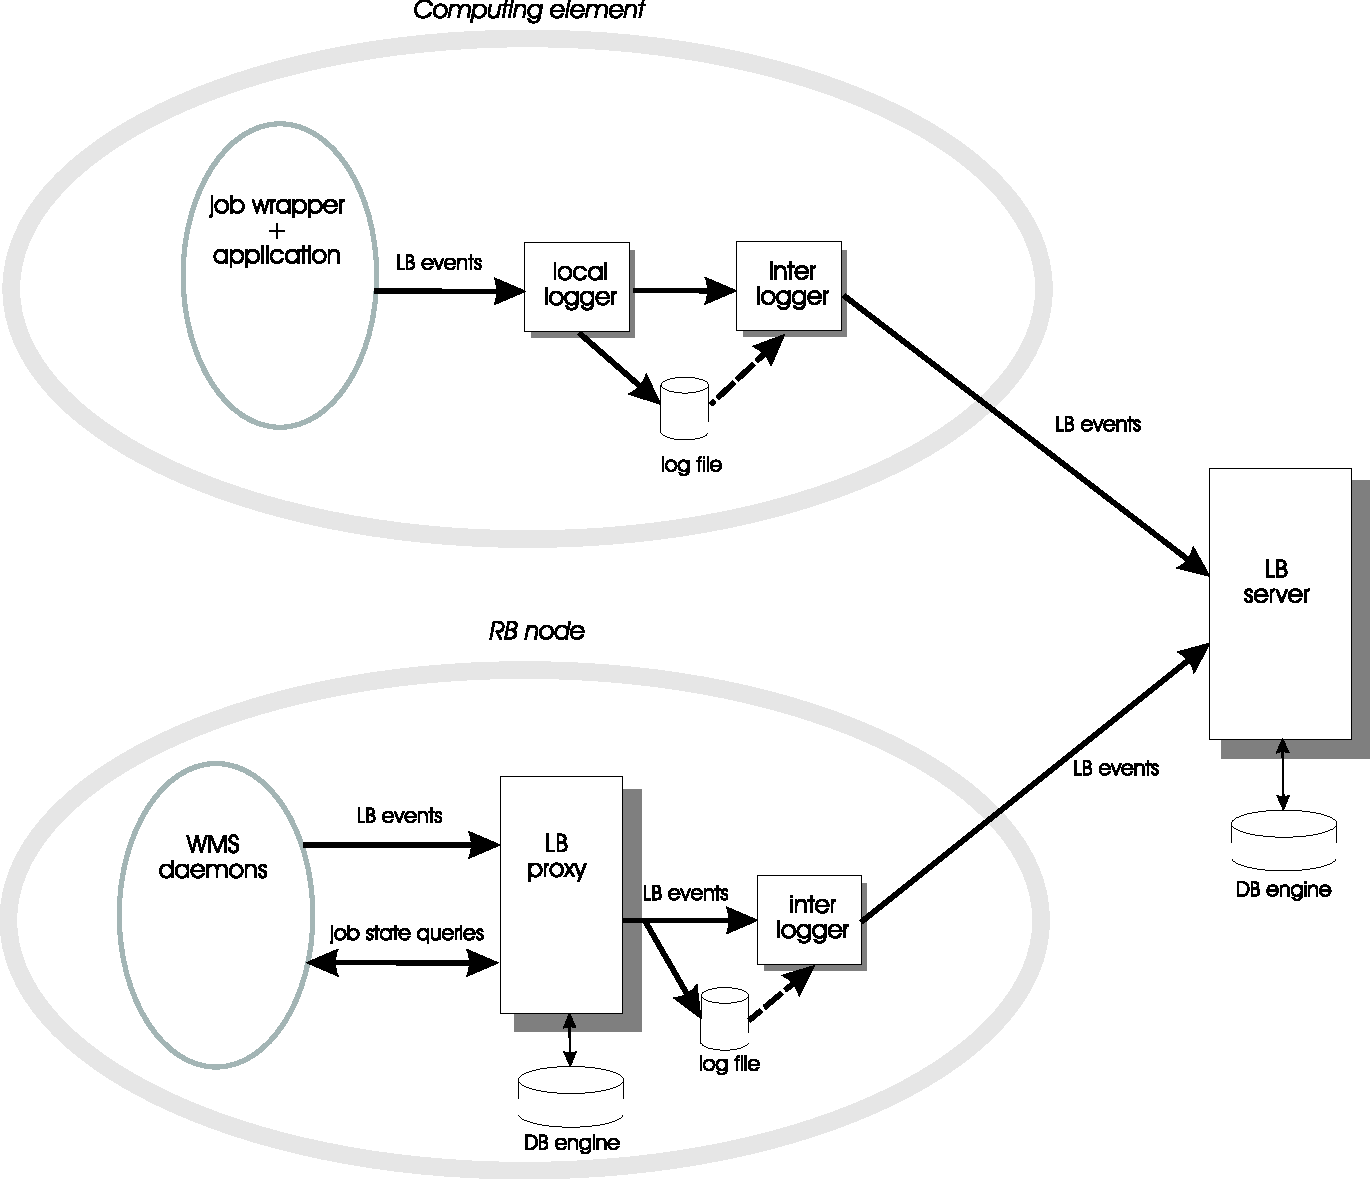
\includegraphics[width=.67\hsize]{LB-components-gather}
\caption{Components involved in gathering and transfering \LB events}
\label{f:comp-gather}
\end{figure}

\begin{figure}[ht]
\centering
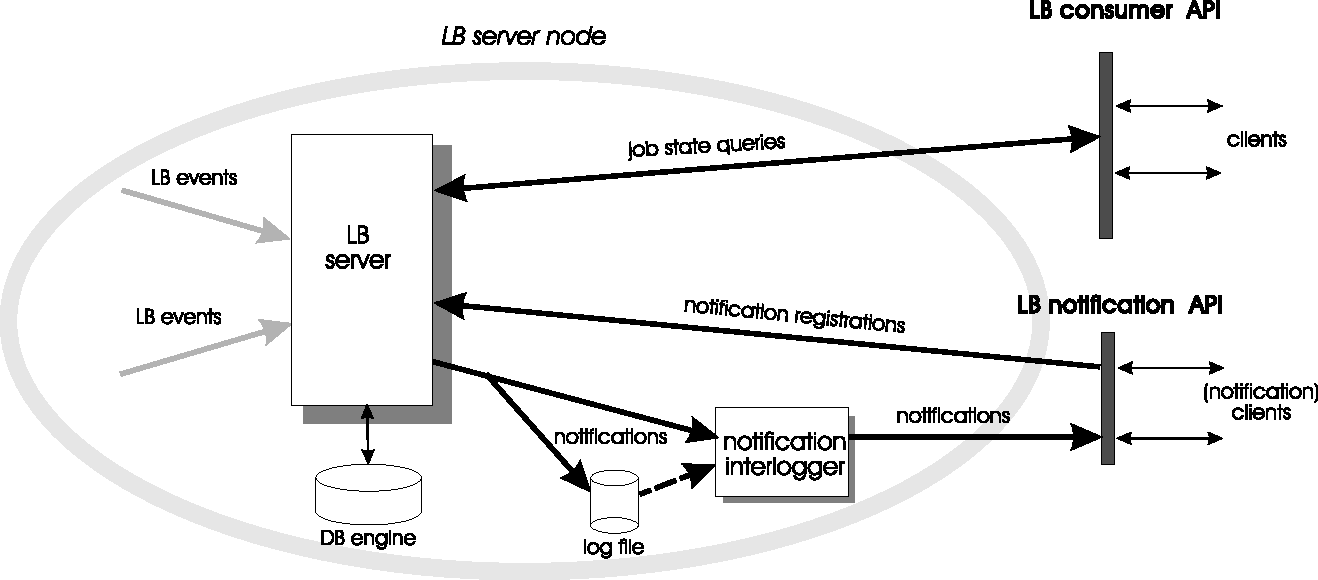
\includegraphics[width=.67\hsize]{LB-components-query}
\caption{\LB queries and notifications}
\label{f:comp-query}
\end{figure}

\TODO{uplne to same (ty components) mame i v UG; chceme to tady duplikovat? 
zvlast kdyz v odstavci nad tim se pise, ze uz je to popsane v UG}
\input components


\subsection{Deployment scenarios}

\TODO{salvet}

\TODO{jakou zatez ktery snese}

\subsubsection{Standalone \LB server}

\subsubsection{Hybrid \LB server-proxy}

Jen 2.0

\subsubsection{\LB server on WMS node}
Highly obsolete and inefficient \dots
